\documentclass{scrartcl}

\usepackage{amsmath}
\usepackage{array}
\usepackage{bytefield}
\usepackage{fontspec}
\usepackage{gitinfo2}
\usepackage{graphicx}
\usepackage{hyperref}
\usepackage{listings}
\usepackage{microtype}
\usepackage{polyglossia}
\usepackage{scrlayer-scrpage}
\usepackage{xcolor}

\linespread{1.3}

\setmainlanguage{lithuanian}

\addtokomafont{disposition}{\rmfamily}

\setmainfont{TeX Gyre Termes}
\setmonofont{TeX Gyre Cursor}

\ohead{Release \gitDescribe\ (\gitCommitterDate)}
\cfoot*{\pagemark}

\newcolumntype{?}{!{\vrule width 1pt}}

\definecolor{lightgray}{gray}{0.8}

\setlength{\headheight}{\baselineskip}
\setlength{\footheight}{\baselineskip}

\lstset{
    basicstyle = \footnotesize\ttfamily,%
    escapeinside = {/*}{*/},%
    firstnumber = 1,%
    numbers = left%
}

\graphicspath{{images/}}

\PolyglossiaSetup{lithuanian}{indentfirst=true}

\begin{document}
    \newcommand{\instr}[3]{\subparagraph{\makebox[6em][l]{\texttt{#1}}} (\texttt{#2})\par#3\par}
    \begin{titlepage}
        \begin{center}
            VILNIAUS UNIVERSITETAS \\
            MATEMATIKOS IR INFORMATIKOS FAKULTETAS \\
            \vspace{4cm}
            \Large\textbf{Virtualios ir realios mašinos projektas}
        \end{center}
        \vspace{4cm}
        \begin{flushright}
            \begin{tabular}[t]{l}
                Atliko: 3 kurso studentai \\
                Tautvydas Baliukynas \\
                Edvinas Gervelis \\
                Ernestas Kulik \\
                Justinas Valatkevičius
            \end{tabular}
        \end{flushright}
        \vspace*{\fill}
        \begin{center}
            \large{Vilnius \\ 2018}
        \end{center}
    \end{titlepage}

    \section{Sistemos procesai}
    Kokie procesai sudaro sistemą,
      \subsection{Procesų būsenos}
        Procesas visą savo gyvavimo laikotarpį būtinai yra vienoje iš išvardintų būsenų:
          \begin{itemize}
              \item \textbf{Vykdomas} - procesas turi procesorių
              \item \textbf{Blokuotas} - procesas prašo kurio nors resurso, išskyrus procesorių
              \item \textbf{Pasiruošęs} - procesui trūksta vienintelio resurso - procesoriaus
              \item \textbf{Sustabdytas} - procesą sustabdė kažkuris kitas procesas
          \end{itemize}
      \subsubsection{Procesų būsenų kaita}
        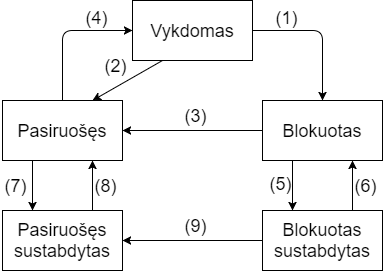
\includegraphics[width=\textwidth]{Process_state}
        \begin{enumerate}
          \item Vykdomas procesas negavo prašomo resurso
          \item Iš vykdomo proceso sistema atima procesorių dėl kokios nors kitos priežasties
          \item Blokuotas procesas gauna reikalingą resursą
          \item Pasiruošęs procesas gauna procesorių
          \item Einamasis procesas sustabdo procesą, kuris buvo užsiblokavęs
          \item Einamasis procesas nuima sustabdymo būsena
          \item Einamasis procesas sustabdo procesą, kuris buvo pasiruošęs
          \item Einamasis procesas nuima sustabdymo būseną
          \item Užsiblokavęs sustabdytas procesas gauna reikalingą resursą
        \end{enumerate}
      \subsection{Procesų kūrimas}
      Procesai yra skirstomi į sisteminius ir vartotojo. Sisteminiai procesai yra sukuriami sistemos darbo pradžioje. Juos sukuria procesas \textbf{StartStop}. Vartotojo procesai yra sukuriami sisteminių procesų. Bendra procesų kūrimo schema:
      \begin{center}
        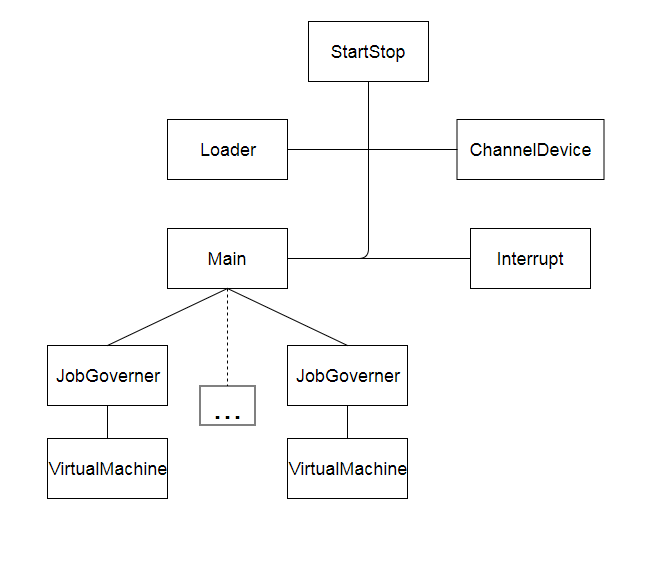
\includegraphics[scale=0.65]{Process_creation}
      \end{center}
      \subsection{Vartotojo programos patekimas į sistemą}
      \begin{center}
        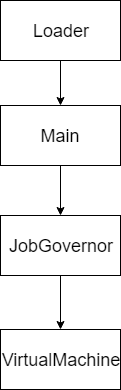
\includegraphics[scale=1]{Program_load}
      \end{center}
      Kol vartotojo programa iš baitų išorinėje atmintyje tampa procesų operacinėje sistemoje, jai tenka pereiti kelis etapus. Visų pirma yra kviečiamas procesas Loader, kuris iš išorinės atminties perskaito užduoties programą, kurią konvertuoja į procesoriui suprantamą formatą ir siunčia pranešimą procesui Main, kuris sukuria po naują JobGoverner procesą kiekvienai vartojo užduočiai. Galiausiai JobGoverner sukuria VirtualMachine procesą, kuris jau gali vykdyti vartojo programą.

      \subsection{Procesų veikimas}
      \subsubsection{StartStop}
        \begin{center}
          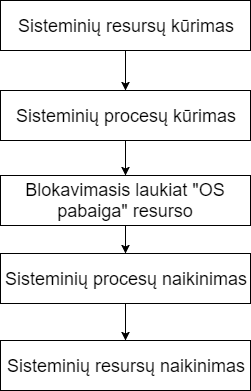
\includegraphics[scale=1]{StartStop}
        \end{center}
      \subsubsection{Loader}
        \begin{center}
          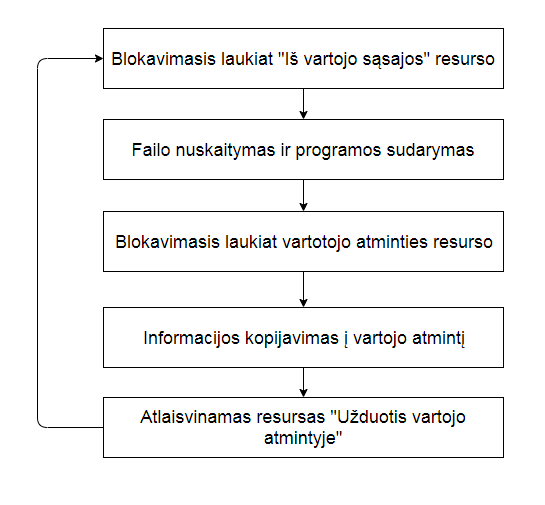
\includegraphics[scale=1]{Loader}
        \end{center}
      \subsubsection{Main}
        \begin{center}
          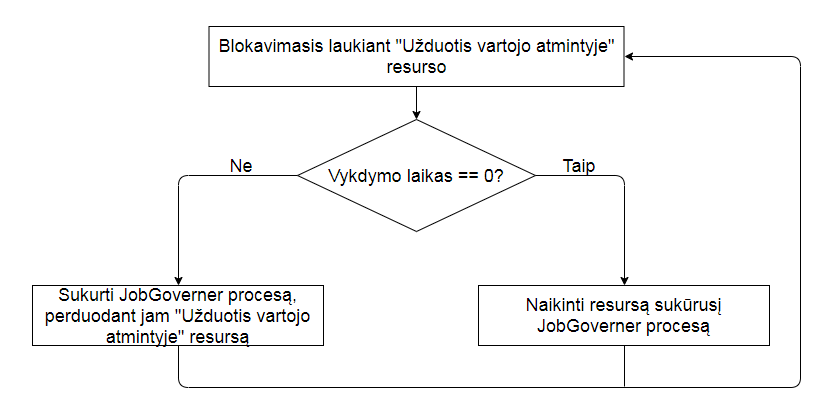
\includegraphics[scale=0.65]{Main}
        \end{center}
      \subsubsection{Interrupt}
        \begin{center}
          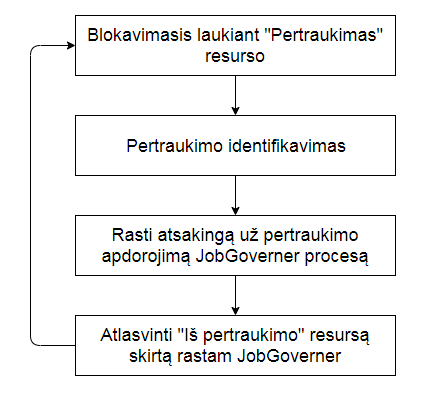
\includegraphics[scale=1]{Interrupt}
        \end{center}
      \subsubsection{ChannelDevice}
        \begin{center}
          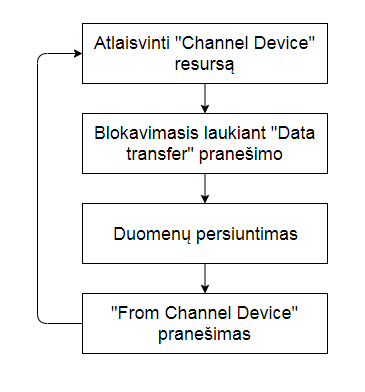
\includegraphics[scale=1]{ChannelDevice}
        \end{center}

      \subsubsection{JobGoverner}
        \begin{center}
          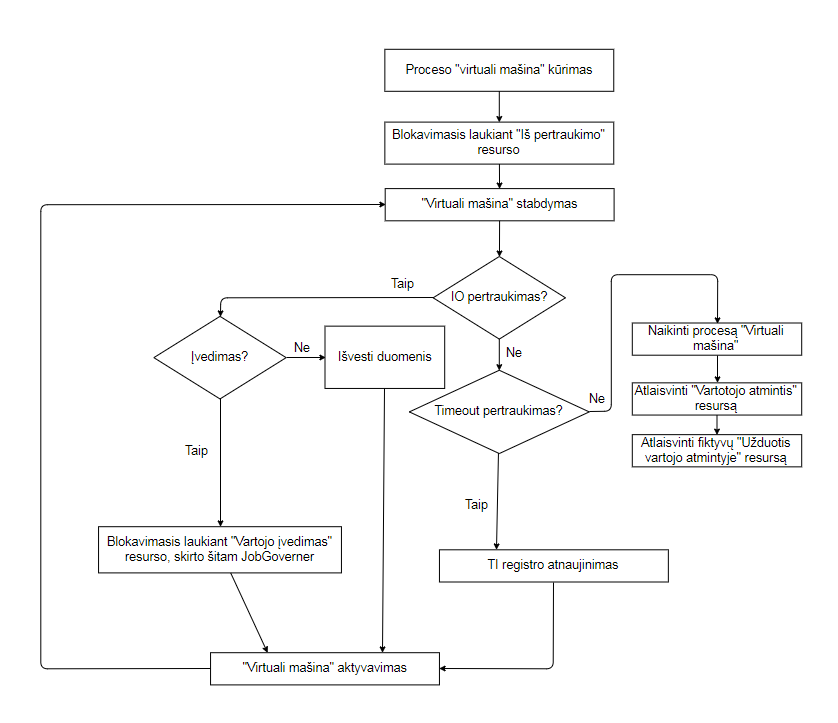
\includegraphics[width=\textwidth]{JobGoverner}
        \end{center}

      \subsubsection{VirtualMachine}
        \begin{center}
          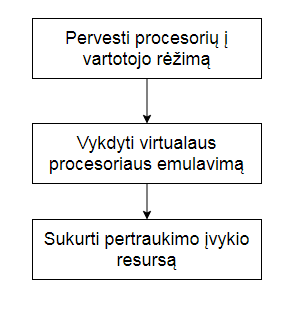
\includegraphics[scale=1]{VirtualMachine}
        \end{center}


    \section{Procesų paskirtis}
    Kokia procesų paskirtis
    \section{Procesų veikimas}
    Kaip veikia procesai
    \section{Resursai}
    Aprašyti, kokius resursus kuria ir kokių laukia procesai
      \subsection{Resursų paskirstytojas}
        \subsubsection{Planuotojas}
        Procesorius iš esmės yra vienas iš sistemos resursų, tačiau, šio resurso svarba sistemoje yra milžiniška, todėl procesorius turi savo atskirą resursų paskirstytoją - planuotoją.
        \par
        Planuotojo pagrindinė užduotis yra skirstyti procesorių sisteminiams ir vartotojo procesams. Skirstymas remiasi procesų prioritetais - planuotojas stengiasi procesorių atiduoti procesui, kurio prioritetas yra aukščiausias.
        \par
        Plantuojo veikimas pagrįstas šia schema:
        \begin{center}
          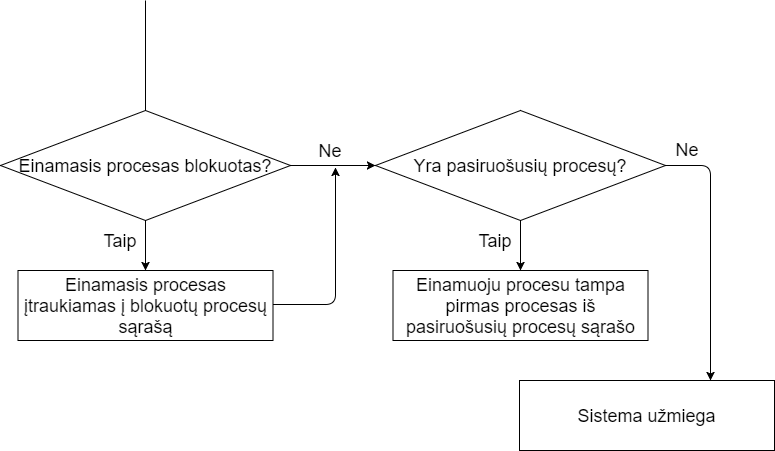
\includegraphics[width=\textwidth]{Planner}
        \end{center}
        Žingsnis, kurio metu procesas iš pasiruošusių procesų sąrašo tampa einamuoju procesu susideda iš tokių veiksmų:
        \begin{enumerate}
          \item Išsaugoma einamojo proceso aplinka, kad ateityje būtų įmanoma pratęsti vykdytą procesą
          \item Užkraunama naujo einamojo proceso aplinka
          \item Naujas einamasis procesas pažymimas kaip einamasis
        \end{enumerate}

    \section{Realios mašinos įrenginių valdymas}
    Aprašyti, kaip OS valdo realios mašinos įrenginius ir kada tai vyksta
        \begin{thebibliography}{999}
            \bibitem{}
                Giedrius Šiaulys,
                Magistro darbas. Mokomoji operacinė sistema,
                2003.
        \end{thebibliography}
    \end{document}
